% Options for packages loaded elsewhere
\PassOptionsToPackage{unicode}{hyperref}
\PassOptionsToPackage{hyphens}{url}
%
\documentclass[
  11pt,
  ignorenonframetext,
  aspectratio=169,
]{beamer}
\usepackage{pgfpages}
\setbeamertemplate{caption}[numbered]
\setbeamertemplate{caption label separator}{: }
\setbeamercolor{caption name}{fg=normal text.fg}
\beamertemplatenavigationsymbolsempty
% Prevent slide breaks in the middle of a paragraph
\widowpenalties 1 10000
\raggedbottom
\setbeamertemplate{part page}{
  \centering
  \begin{beamercolorbox}[sep=16pt,center]{part title}
    \usebeamerfont{part title}\insertpart\par
  \end{beamercolorbox}
}
\setbeamertemplate{section page}{
  \centering
  \begin{beamercolorbox}[sep=12pt,center]{part title}
    \usebeamerfont{section title}\insertsection\par
  \end{beamercolorbox}
}
\setbeamertemplate{subsection page}{
  \centering
  \begin{beamercolorbox}[sep=8pt,center]{part title}
    \usebeamerfont{subsection title}\insertsubsection\par
  \end{beamercolorbox}
}
\AtBeginPart{
  \frame{\partpage}
}
\AtBeginSection{
  \ifbibliography
  \else
    \frame{\sectionpage}
  \fi
}
\AtBeginSubsection{
  \frame{\subsectionpage}
}
\usepackage{lmodern}
\usepackage{amssymb,amsmath}
\usepackage{ifxetex,ifluatex}
\ifnum 0\ifxetex 1\fi\ifluatex 1\fi=0 % if pdftex
  \usepackage[T1]{fontenc}
  \usepackage[utf8]{inputenc}
  \usepackage{textcomp} % provide euro and other symbols
\else % if luatex or xetex
  \usepackage{unicode-math}
  \defaultfontfeatures{Scale=MatchLowercase}
  \defaultfontfeatures[\rmfamily]{Ligatures=TeX,Scale=1}
\fi
% Use upquote if available, for straight quotes in verbatim environments
\IfFileExists{upquote.sty}{\usepackage{upquote}}{}
\IfFileExists{microtype.sty}{% use microtype if available
  \usepackage[]{microtype}
  \UseMicrotypeSet[protrusion]{basicmath} % disable protrusion for tt fonts
}{}
\makeatletter
\@ifundefined{KOMAClassName}{% if non-KOMA class
  \IfFileExists{parskip.sty}{%
    \usepackage{parskip}
  }{% else
    \setlength{\parindent}{0pt}
    \setlength{\parskip}{6pt plus 2pt minus 1pt}}
}{% if KOMA class
  \KOMAoptions{parskip=half}}
\makeatother
\usepackage{xcolor}
\IfFileExists{xurl.sty}{\usepackage{xurl}}{} % add URL line breaks if available
\IfFileExists{bookmark.sty}{\usepackage{bookmark}}{\usepackage{hyperref}}
\hypersetup{
  pdftitle={Restricted Randomization Beyond Permuted Blocks},
  pdfauthor={Kevin Venner, Diane Uschner},
  hidelinks,
  pdfcreator={LaTeX via pandoc}}
\urlstyle{same} % disable monospaced font for URLs
\newif\ifbibliography
\setlength{\emergencystretch}{3em} % prevent overfull lines
\providecommand{\tightlist}{%
  \setlength{\itemsep}{0pt}\setlength{\parskip}{0pt}}
\setcounter{secnumdepth}{-\maxdimen} % remove section numbering
\usepackage{rwg-theme}
\usepackage{booktabs}
\usepackage{longtable}
\usepackage{array}
\usepackage{multirow}
\usepackage{wrapfig}
\usepackage{float}
\usepackage{colortbl}
\usepackage{pdflscape}
\usepackage{tabu}
\usepackage{threeparttable}
\usepackage{threeparttablex}
\usepackage[normalem]{ulem}
\usepackage{makecell}
\usepackage{xcolor}
\newlength{\cslhangindent}
\setlength{\cslhangindent}{1.5em}
\newenvironment{cslreferences}%
  {\setlength{\parindent}{0pt}%
  \everypar{\setlength{\hangindent}{\cslhangindent}}\ignorespaces}%
  {\par}

\title{Restricted Randomization Beyond Permuted Blocks}
\subtitle{SCT Arizona 2026}
\author{Kevin Venner, Diane Uschner}
\date{May 2026}

\begin{document}
\frame{\titlepage}

\hypertarget{introduction}{%
\section{Introduction}\label{introduction}}

\begin{frame}{Outline}
\protect\hypertarget{outline}{}
\begin{enumerate}
\tightlist
\item
  Why block randomization is increasingly challenged
\item
  Mathematical perspective on restricted randomization
\item
  Maximum tolerated imbalance (MTI) framework
\item
  Practical alternatives to permuted block randomization
\item
  Predictability under equal MTI constraints
\item
  Implementation and take-home messages
\end{enumerate}
\end{frame}

\hypertarget{why-rethink-permuted-block-randomization}{%
\section{Why Rethink Permuted Block
Randomization?}\label{why-rethink-permuted-block-randomization}}

\begin{frame}{Block Randomization Under Challenge}
\protect\hypertarget{block-randomization-under-challenge}{}
\begin{itemize}
\tightlist
\item
  Permuted block randomization has been widely used for decades because
  it controls treatment imbalance tightly.
\item
  In modern trials, that strong control can come at a cost: higher
  allocation predictability.
\item
  Predictability increases the risk of selection bias when treatment
  history can be partially inferred.
\item
  The core question is no longer only balance, but balance versus
  randomness and robustness.
\end{itemize}
\end{frame}

\begin{frame}{Dynamic Allocation and Current Trial State}
\protect\hypertarget{dynamic-allocation-and-current-trial-state}{}
\begin{itemize}
\tightlist
\item
  Treatment assignment is sequential and depends on the current state of
  the trial.
\item
  In blocked and stratified designs, assignment probabilities are
  influenced by current within-block imbalance.
\item
  Stratification adds another dynamic layer because covariate strata
  evolve over enrollment.
\item
  This dynamic dependence is shared by many restricted randomization
  designs, not only permuted blocks.
\end{itemize}
\end{frame}

\hypertarget{mathematical-framing}{%
\section{Mathematical Framing}\label{mathematical-framing}}

\begin{frame}{Restricted Randomization as a Dynamic Process}
\protect\hypertarget{restricted-randomization-as-a-dynamic-process}{}
\begin{itemize}
\tightlist
\item
  Restricted randomization can be viewed as a stochastic process on
  imbalance states.
\item
  At each step, the design updates assignment probabilities using
  current history.
\item
  Design properties are therefore path-dependent, not just determined by
  the final sample size.
\item
  This framing helps compare designs on predictability, imbalance, and
  inferential performance.
\end{itemize}
\end{frame}

\begin{frame}{Dependence on Treatment Balance and Stratum State}
\protect\hypertarget{dependence-on-treatment-balance-and-stratum-state}{}
\begin{itemize}
\tightlist
\item
  Let \(D_i = N_C(i)-N_E(i)\) denote treatment imbalance after subject
  \(i\).
\item
  In stratified settings, each stratum has its own imbalance trajectory.
\item
  The next assignment probability is a function of the current imbalance
  state (and potentially stratum).
\item
  Strong correction toward \(D_i=0\) improves balance but can make
  assignments easier to guess.
\end{itemize}
\end{frame}

\hypertarget{mti-based-design-strategy}{%
\section{MTI-Based Design Strategy}\label{mti-based-design-strategy}}

\begin{frame}{Maximum Tolerated Imbalance (MTI)}
\protect\hypertarget{maximum-tolerated-imbalance-mti}{}
\begin{itemize}
\tightlist
\item
  MTI designs enforce a hard boundary on allowable imbalance:
  \(|D_i| \leq b\).
\item
  Inside the boundary, randomization is flexible; at the boundary,
  correction is enforced.
\item
  MTI provides a transparent tuning parameter for the balance-randomness
  trade-off.
\item
  This gives a common framework to compare procedures at the same
  imbalance tolerance.
\end{itemize}
\end{frame}

\begin{frame}{Visualization of the MTI tunnel}
\protect\hypertarget{visualization-of-the-mti-tunnel}{}
\center

\includegraphics[width=0.8\linewidth]{slides_SCT_Uschner_files/figure-beamer/unnamed-chunk-1-1}
\end{frame}

\begin{frame}{Releasing Enforced Block-End Perfect Balance}
\protect\hypertarget{releasing-enforced-block-end-perfect-balance}{}
\begin{itemize}
\tightlist
\item
  Permuted blocks force deterministic structure near the end of each
  block.
\item
  MTI-based alternatives relax this block-end perfect balance
  requirement.
\item
  The result is lower predictability while still controlling worst-case
  imbalance.
\item
  In practice, this can reduce selection bias risk without sacrificing
  operational simplicity.
\end{itemize}
\end{frame}

\hypertarget{alternative-designs}{%
\section{Alternative Designs}\label{alternative-designs}}

\begin{frame}{Maximal Procedure}
\protect\hypertarget{maximal-procedure}{}
\begin{itemize}
\tightlist
\item
  The maximal procedure is an MTI-constrained restricted randomization
  design with equi-probable randomization sequences and the contraint of
  final group balance
\item
  It maximizes randomness subject to the imbalance bound, avoiding fixed
  block structure.
\item
  Under matched MTI constraints, it is less predictable than permuted
  block randomization.
\item
  It is a practical option when allocation concealment and
  anti-predictability as well as exact final balance are priorities.
\item
  Implementation requires knowing the target group sizes in advance.
\end{itemize}
\end{frame}

\begin{frame}{Big Stick Design}
\protect\hypertarget{big-stick-design}{}
\begin{itemize}
\tightlist
\item
  Big Stick Design randomizes freely until the MTI boundary is reached.
\item
  At the boundary, assignment is forced only to move imbalance back
  toward zero.

  \begin{itemize}
  \tightlist
  \item
    As a result, sequences are not equi-probable, but the design is less
    predictable than permuted blocks.
  \end{itemize}
\item
  This yields less deterministic behavior than permuted blocks while
  preserving MTI control.
\item
  Operationally, it is straightforward to implement with centralized
  randomization tools.
\end{itemize}
\end{frame}

\begin{frame}{Implementation Simplicity and Practical Use}
\protect\hypertarget{implementation-simplicity-and-practical-use}{}
\begin{itemize}
\tightlist
\item
  Big Stick and maximal procedure designs are feasible for routine trial
  operations.
\item
  They can be pre-specified in SAP/protocol language similarly to
  existing restricted methods.
\item
  Implementation burden is typically low with modern IWRS/IRT
  infrastructure.
\item
  Design choice should be justified by expected bias risk, not
  convenience alone.
\end{itemize}
\end{frame}

\hypertarget{predictability-evidence}{%
\section{Predictability Evidence}\label{predictability-evidence}}

\begin{frame}{Equal-MTI Comparisons Across Designs}
\protect\hypertarget{equal-mti-comparisons-across-designs}{}
\begin{itemize}
\tightlist
\item
  Fair comparisons should match designs on the same MTI level.

  \begin{itemize}
  \tightlist
  \item
    For the permuted block design, the MTI is half the block size (e.g.,
    MTI=2 for block size 4).
  \end{itemize}
\item
  Under equal MTI, designs can differ meaningfully in allocation
  predictability.
\item
  Literature shows that predictability is not an unavoidable consequence
  of imbalance control.
\item
  This supports selecting designs by properties, not by historical
  default.
\end{itemize}
\end{frame}

\begin{frame}{Notation}
\protect\hypertarget{notation}{}
Let \(N\) be the total sample size, \(i\) the patient index, and
\(t \in \Omega:=\{0,1\}^N\) a randomization sequence, where

\[
t_i = \begin{cases}
1 & i \text{ is allocated to } E\\
0 & i \text{ is allocated to } C
\end{cases}
\]

We call \(\Omega\) the set of all sequences. For a sequence \(t\),

\begin{align*}
N_E(i) &:= N_E(t,i) := \sum_{j=1}^i t_j \\
N_C(i) &:= N_C(t,i) := i - \sum_{j=1}^i t_j
\end{align*}

define the number of patients in groups \(E\) and \(C\) after \(i\)
allocations.
\end{frame}

\begin{frame}{Predictability Metric: Correct Guesses}
\protect\hypertarget{predictability-metric-correct-guesses}{}
\begin{itemize}
\item
  In the situation of third order selection bias, the investigator can
  count \(N_E(i)\) and \(N_C(i)\) respectively.
\item
  Under the assumption that \(N_E(N) = N_C(N)\) for all \(t \in \Omega\)
  it makes sense for the investigator to guess \[g(t_{i+1})= 
          \begin{cases}
          0               & N_E(i) > N_C(i)\\
          Ber(0.5)  & N_E(i) = N_C(i)\\
          1               & N_E(i) < N_C(i),
          \end{cases}\] following the so called \emph{convergence
  strategy}.
\end{itemize}

{(Blackwell and Hodges 1957)}
\end{frame}

\begin{frame}{Visualization Correct Guesses}
\protect\hypertarget{visualization-correct-guesses}{}
\begin{center}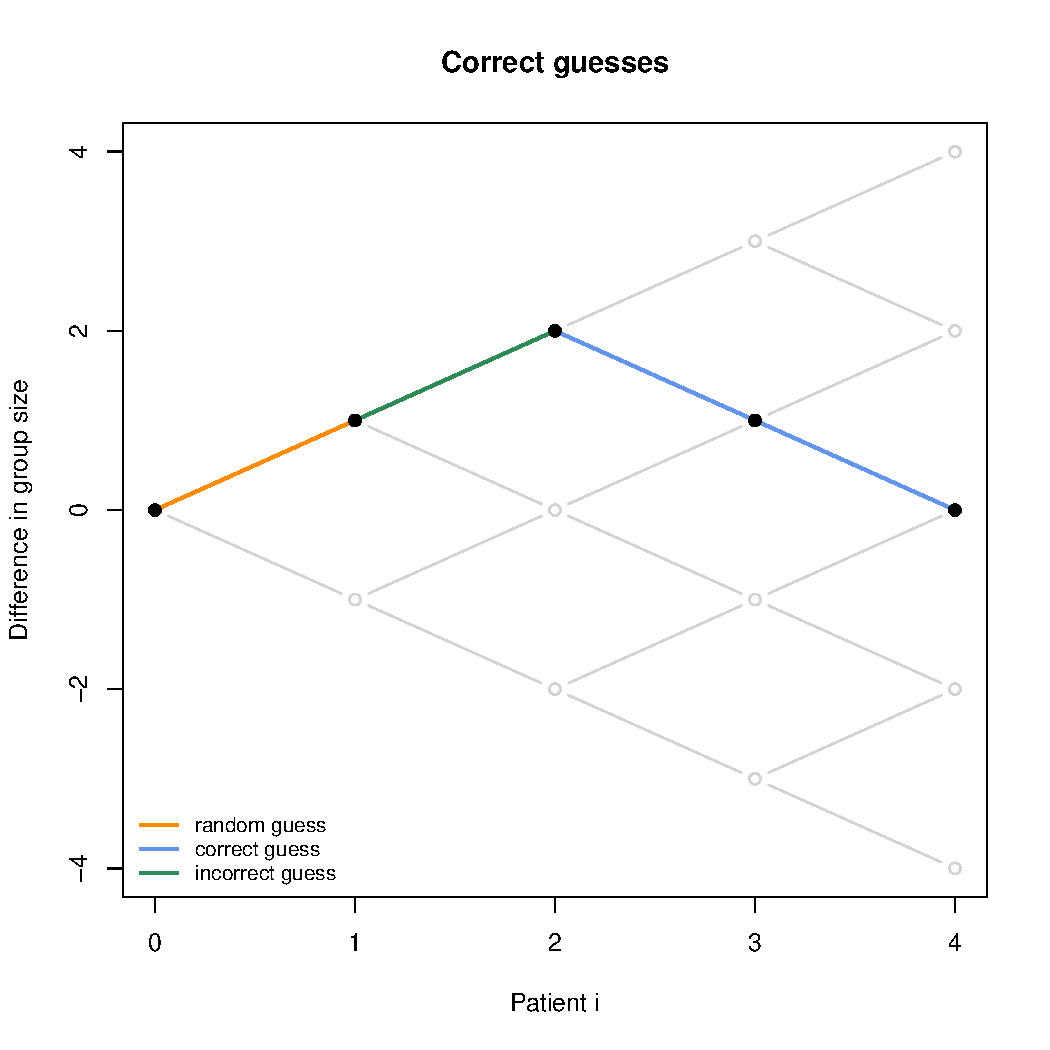
\includegraphics[height=0.8\textheight]{./graphics/correct-guesses} \end{center}
\end{frame}

\begin{frame}{Design Comparison with respect to Predictability}
\protect\hypertarget{design-comparison-with-respect-to-predictability}{}
\includegraphics[height=0.8\textheight]{slides_SCT_Uschner_files/figure-beamer/pred-compare-plot-1}
\end{frame}

\begin{frame}{Why Permuted Block Is Most Predictable Under MTI}
\protect\hypertarget{why-permuted-block-is-most-predictable-under-mti}{}
\begin{itemize}
\tightlist
\item
  With fixed block structure, remaining allocations become progressively
  constrained.
\item
  Near block completion, upcoming assignments can often be inferred with
  high probability.
\item
  Theoretical and empirical work shows permuted blocks are most
  predictable among equal-MTI designs.
\item
  Therefore, permuted blocks may be inferior when minimizing
  predictability is a design priority.
\end{itemize}
\end{frame}

\hypertarget{conclusions}{%
\section{Conclusions}\label{conclusions}}

\begin{frame}{Key Messages}
\protect\hypertarget{key-messages}{}
\begin{itemize}
\tightlist
\item
  Balance control and allocation unpredictability should be considered
  jointly.
\item
  Under equal MTI, permuted blocks are generally more predictable than
  alternatives.
\item
  Big Stick and maximal procedure are practical, implementable, and
  often preferable options.
\item
  Moving beyond default blocked randomization can improve design
  robustness.
\end{itemize}
\end{frame}

\begin{frame}{Discussion}
\protect\hypertarget{discussion}{}
\begin{itemize}
\tightlist
\item
  Which trial settings in our portfolio are most vulnerable to selection
  bias?
\item
  What MTI level is acceptable from a clinical and operational
  perspective?
\item
  Should we update internal default randomization recommendations beyond
  permuted blocks?
\end{itemize}

\hypertarget{refs}{}
\begin{cslreferences}
\leavevmode\hypertarget{ref-Blackwell1957}{}%
Blackwell, D., and J. Hodges. 1957. ``Design for the Control of
Selection Bias.'' \emph{Annals of Mathematical Statistics} 25: 449--60.
\end{cslreferences}
\end{frame}

\end{document}
